\documentclass[11pt,a4paper]{article}
\usepackage[margin=2.0cm,top=2.2cm,bottom=2.2cm]{geometry}
\usepackage{amsmath,amssymb}
\usepackage{enumitem}
\usepackage{booktabs}
\usepackage{graphicx}
\graphicspath{{../../presentation/assets/}{./}}
\usepackage{float}
\usepackage{placeins}
\usepackage{xcolor}
\usepackage{caption}
\captionsetup{font=small,labelfont=bf}
\usepackage[colorlinks=true, linkcolor=blue!45!black, urlcolor=blue!45!black, citecolor=blue!45!black]{hyperref}
\usepackage{parskip}
\usepackage{fancyhdr}
\setlength{\headheight}{13.6pt}
\pagestyle{fancy}\fancyhf{}
\lhead{Computational Genomics}\rhead{Hackathon}\cfoot{\thepage}
\renewcommand{\headrulewidth}{0.4pt}
\begin{document}
\begin{center}
  {\Large\bfseries Computational Genomics -- Hackathon}\\[0.4em]
  {\large Does the snRNA-seq evidence for hepatocyte de-zonation survive matched sampling? A re-analysis note}\\[0.7em]
  Roee Tekoah \quad(\href{mailto:roee.tekoah@mail.huji.ac.il}{roee.tekoah@mail.huji.ac.il})\\[0.2em]
  Shira Gelbstein
\end{center}
\vspace{0.4em}

{\small\noindent\textbf{Abstract.~}Gribben et al.\ report that during human chronic liver disease (MASLD) hepatocytes progressively lose their spatial zonation and acquire cholangiocyte-like (biliary) features. We re-examined the single-nucleus RNA-seq evidence for the \emph{progressive de-zonation} part of that claim. The complication we found is structural: \textbf{disease stage is collinear with how the tissue was obtained.} Healthy and end-stage samples are deceased-donor organ tissue (a $\sim$1\,cm$^3$ cube / explant); the F0--F4 disease spectrum is 16-gauge needle biopsy. So ``healthy $\to$ MASLD $\to$ end-stage'' is also ``organ cube $\to$ needle $\to$ explant,'' and a single pooled correlation cannot tell disease from acquisition. After setting aside the source-confounded endpoints and re-testing on the matched needle-biopsy axis --- using raw UMI counts, depth-normalized per nucleus, with the \textbf{donor} ($\sim$47) as the unit of inference --- pericentral/periportal structure is \textbf{preserved across fibrosis F1$\to$cirrhotic F4}. A donor-level pseudobulk differential-expression scan finds no zonation-marker loss; its one signal is a small \textbf{biliary/ductular-marker burden} at F4, more consistent with cholangiocyte ambient RNA plus rare mixed/doublet nuclei (the ductular reaction) than with broad hepatocyte transdifferentiation. We do not claim to overturn the paper; biliary source attribution is \textbf{a lead, not closed.}}\par\vspace{0.5em}

\setcounter{tocdepth}{2}
\begingroup\renewcommand{\contentsname}{\normalsize Contents}{\small\tableofcontents}\endgroup
\vspace{0.6em}

\section{Question and scope}

The published claim has two parts: hepatocytes progressively \emph{lose zonation}, and they acquire \emph{cholangiocyte-like plasticity}. The paper tests de-zonation with a marker--marker correlation (Welch's t-test) pooled across all 47 donors, and confirms plasticity with tissue imaging.

Our question is narrow: \textbf{does the single-nucleus transcriptional evidence for progressive de-zonation survive a matched-source analysis?} Scope: raw snRNA counts only. We do not touch the paper's imaging, immunostaining, protein, organoid, or spatial-architecture evidence --- and we agree with the paper that its strong signal is an end-stage phenomenon. We are not claiming to overturn the full paper.

Zonation means hepatocytes run different programs by lobule position: pericentral (PC, near the central vein) cells favor \emph{GLUL, CYP3A4} and drug-metabolizing enzymes; periportal (PP) cells favor \emph{ASS1, PCK1, HAL, ALDOB} (urea cycle, gluconeogenesis). De-zonation could break this in several distinct ways --- PC cells deplete, zonal genes turn off, cells co-express both programs, the gradient compresses, or the PP:PC balance shifts. Because each failure mode has a different count signature, we tested them separately rather than leaning on one global score.

\section{Data and the key confound}

The dataset is not one homogeneous disease series. Tissue source is tied to stage:

\begin{table}[h]
\centering
\small
\begin{tabular}{lll}
\toprule
Group & Tissue source & Acquisition \\
\midrule
Healthy (n=4) & Deceased-donor organ tissue (one with biliary-stone disease) & $\sim$1\,cm$^3$ organ cube \\
Disease F0--F4 & MASLD/NASH/cirrhosis & 16-gauge end-cut needle biopsy \\
End-stage (n=5) & Explanted cirrhotic organs (left/right/caudate lobes) & Whole-organ explant \\
\bottomrule
\end{tabular}
\caption{The three sampling groups. Both ends of the apparent disease axis are organ tissue; only the F0--F4 middle is needle biopsy.}
\label{tab:groups}
\end{table}

Both \emph{ends} of the apparent disease axis are organ tissue; only the F0--F4 middle is needle biopsy (grounded directly in Paper 1's Methods, \texttt{papers/s41586-024-07465-2.pdf}; see \texttt{reports/SYNTHESIS.md} \S1a). The trajectory ``healthy $\to$ MASLD $\to$ end-stage'' is therefore also an \textbf{acquisition trajectory} --- ischemia, procurement delay, dissociation, organ-cube-vs-needle, and sequencing batch all move together with stage (run almost perfectly predicts tissue source: Cram\'er's V $\approx 0.84$). This is the load-bearing issue: it motivates excluding the ends and re-testing biopsy-only.

\textbf{Figure 1 --- Study design and the source confound} \emph{(schematic; see presentation slide 3)}: a three-group panel showing that disease stage runs collinear with acquisition mode, so a pooled comparison reads a procurement discontinuity as biology. The three sampling groups are laid out in Table~\ref{tab:groups}.

\section{Methods that matter}

Only the choices that explain why our result differs.

\textbf{3.1 Raw counts, not the shipped matrix.} The distributed matrix is an SCT model output (depth squeezed); we extracted real RNA-assay UMI counts. All molecule inference is on raw counts.

\textbf{3.2 Depth-normalized anchor classification.} Each hepatocyte nucleus is down-thinned to a common 1{,}500-UMI budget (binomial thinning, averaged over draws) so detection reflects biology not depth. A marker is ``on'' at $\ge 2$ UMI (ambient-robust). Using strict mutually-exclusive anchors --- PC = \emph{GLUL/CYP3A4}, PP = \emph{ASS1/PCK1/HAL/ALDOB} --- each nucleus is labeled PC, PP, dual, or null. The unit of inference is the \textbf{donor}, never the cell. (This is differential-abundance / composition analysis; we call it ``anchor classification.'')

\textbf{3.3 Donor-level pseudobulk DGE.} Sum each donor's hepatocyte raw UMIs into one count profile; run edgeR (TMM normalization, negative-binomial quasi-likelihood), primary contrast F4-vs-F1 across 38 biopsy donors. Purpose: a genome-wide check for \textbf{non-zonation} programs given that zonation structure is treated as settled --- not a second de-zonation test.

\section{Results}

\subsection{R1 --- The endpoints carry acquisition stress, so we exclude them}
A curated stress module (immediate-early + heat-shock genes), depth-normalized, runs at \textbf{0.074} mean UMIs/nucleus in biopsies, \textbf{0.282} in healthy organ cubes, and \textbf{1.675} in end-stage explants ($\sim$22$\times$ biopsy). The decisive control is cross-lineage: end-stage-vs-biopsy stress is $\sim$18.5$\times$ in hepatocytes and $\sim$18.2$\times$ in \textbf{endothelial cells}, which carry no zonation program. A signal identical in a non-zonated lineage is whole-organ procurement handling, not hepatocyte biology --- and it perturbs exactly the oxygen/Wnt-gradient axis the de-zonation claim rests on. This justifies excluding the source-confounded endpoints from the disease axis.

\begin{figure}[h]
\centering
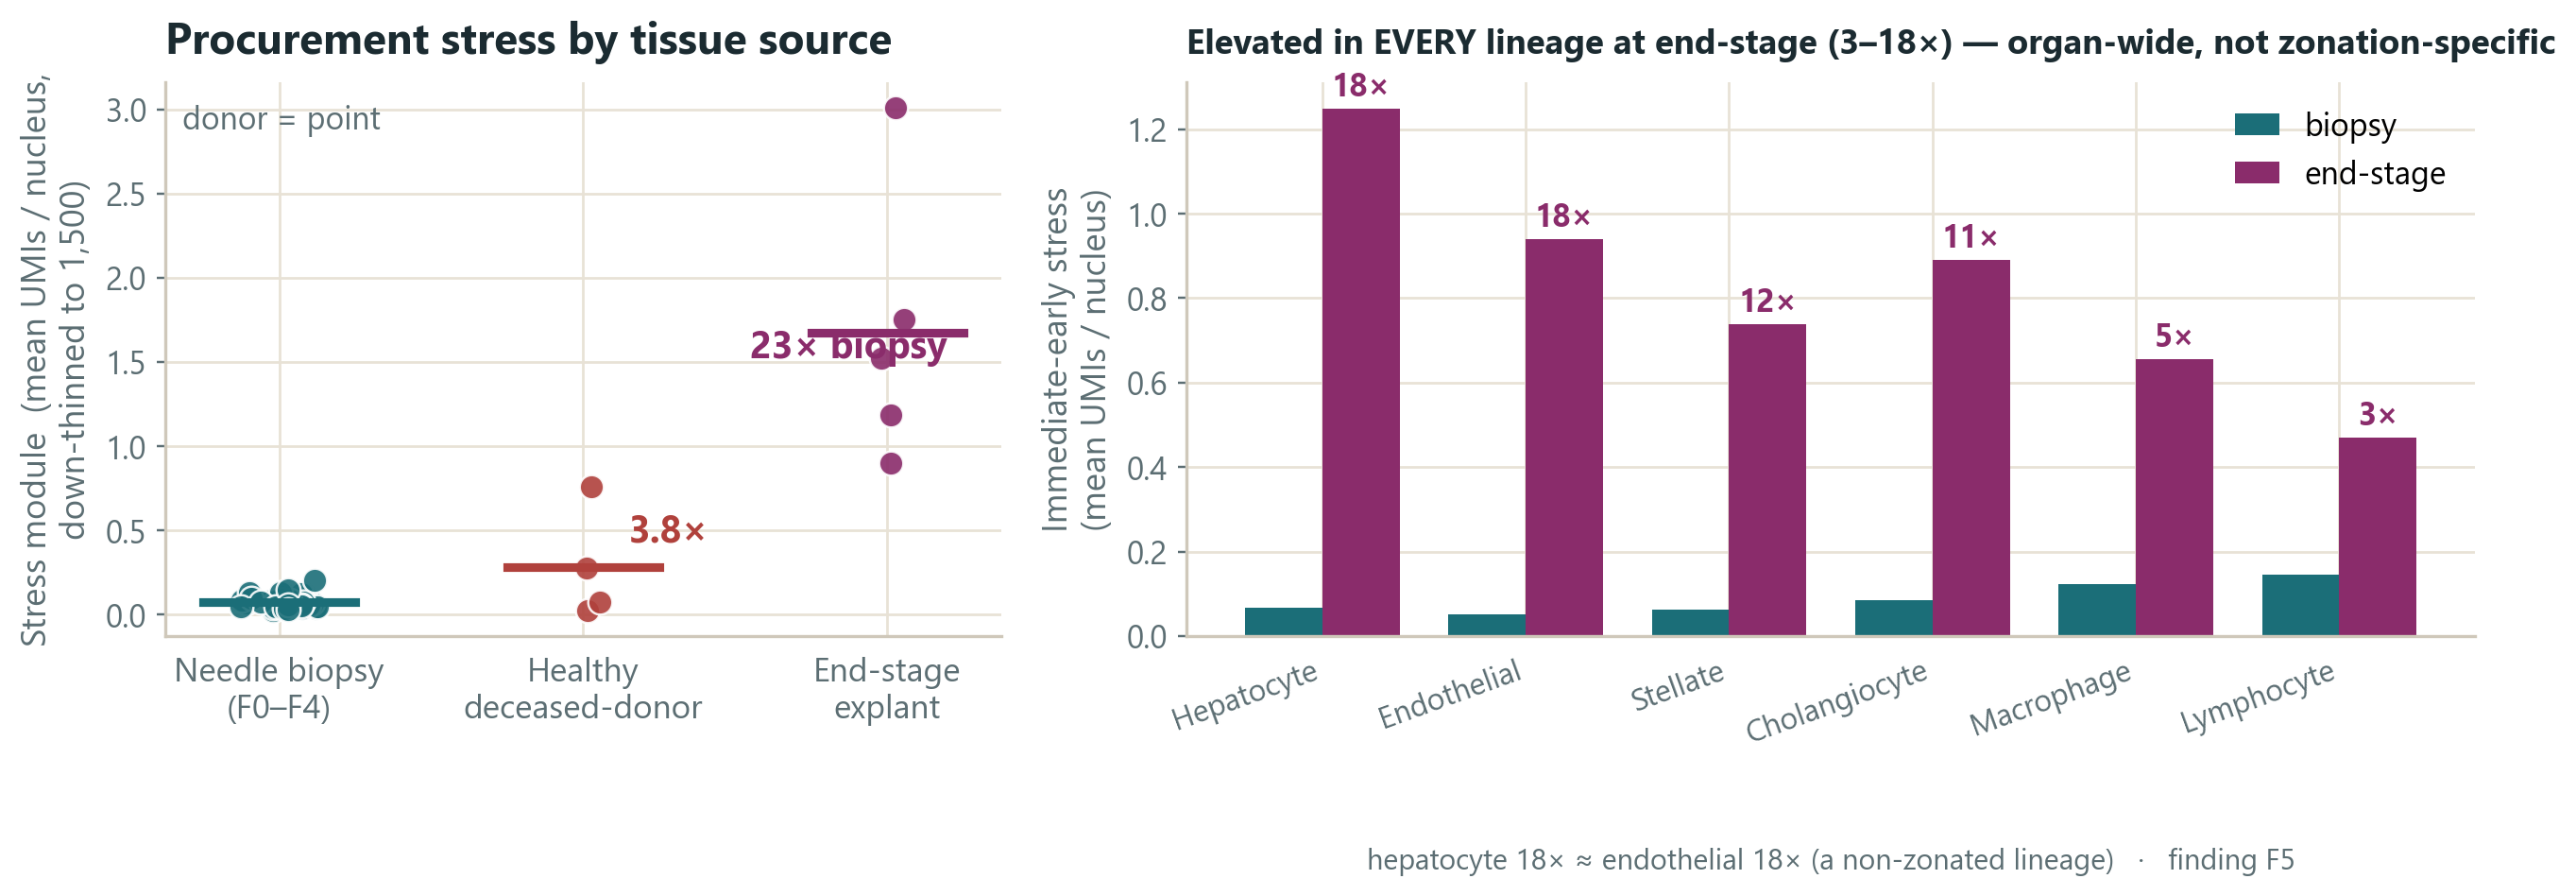
\includegraphics[width=0.8\linewidth]{fig_stress}
\caption{Procurement stress by group and lineage. The endpoints (organ cube, explant) carry an organ-wide acute stress signature; biopsies are uniformly low and flat.}
\label{fig:stress}
\end{figure}

\subsection{R2 --- On the matched biopsy axis, zonation is preserved}
Across F0--F4 needle biopsies the structure holds by every failure mode:
\begin{itemize}[noitemsep]
\item \textbf{Depletion:} PC-anchor fraction 36/19/23/22/21\% (F0--F4) --- flat/non-monotone.
\item \textbf{Co-expression:} the dual fraction looks inflated ($\sim$7--10\%) only at a 1-UMI threshold; at the ambient-robust $\ge 2$-UMI cut it collapses to \textbf{$\sim$0.2--0.6\%} with no trend --- the 1-UMI signal was ambient soup.
\item \textbf{Turn-off:} null fraction flat.
\item \textbf{Composition:} PP:PC ratio 0.62/1.16/1.01/1.10/1.18 --- flat/non-monotone.
\end{itemize}

The poles stay dominant; at most a mild non-monotone middle-ward drift. The null is robust across the full sensitivity grid and a marker-set ladder from 2 to 1{,}637 genes (including Paper 2's own 40 landmark genes).

\begin{figure}[h]
\centering
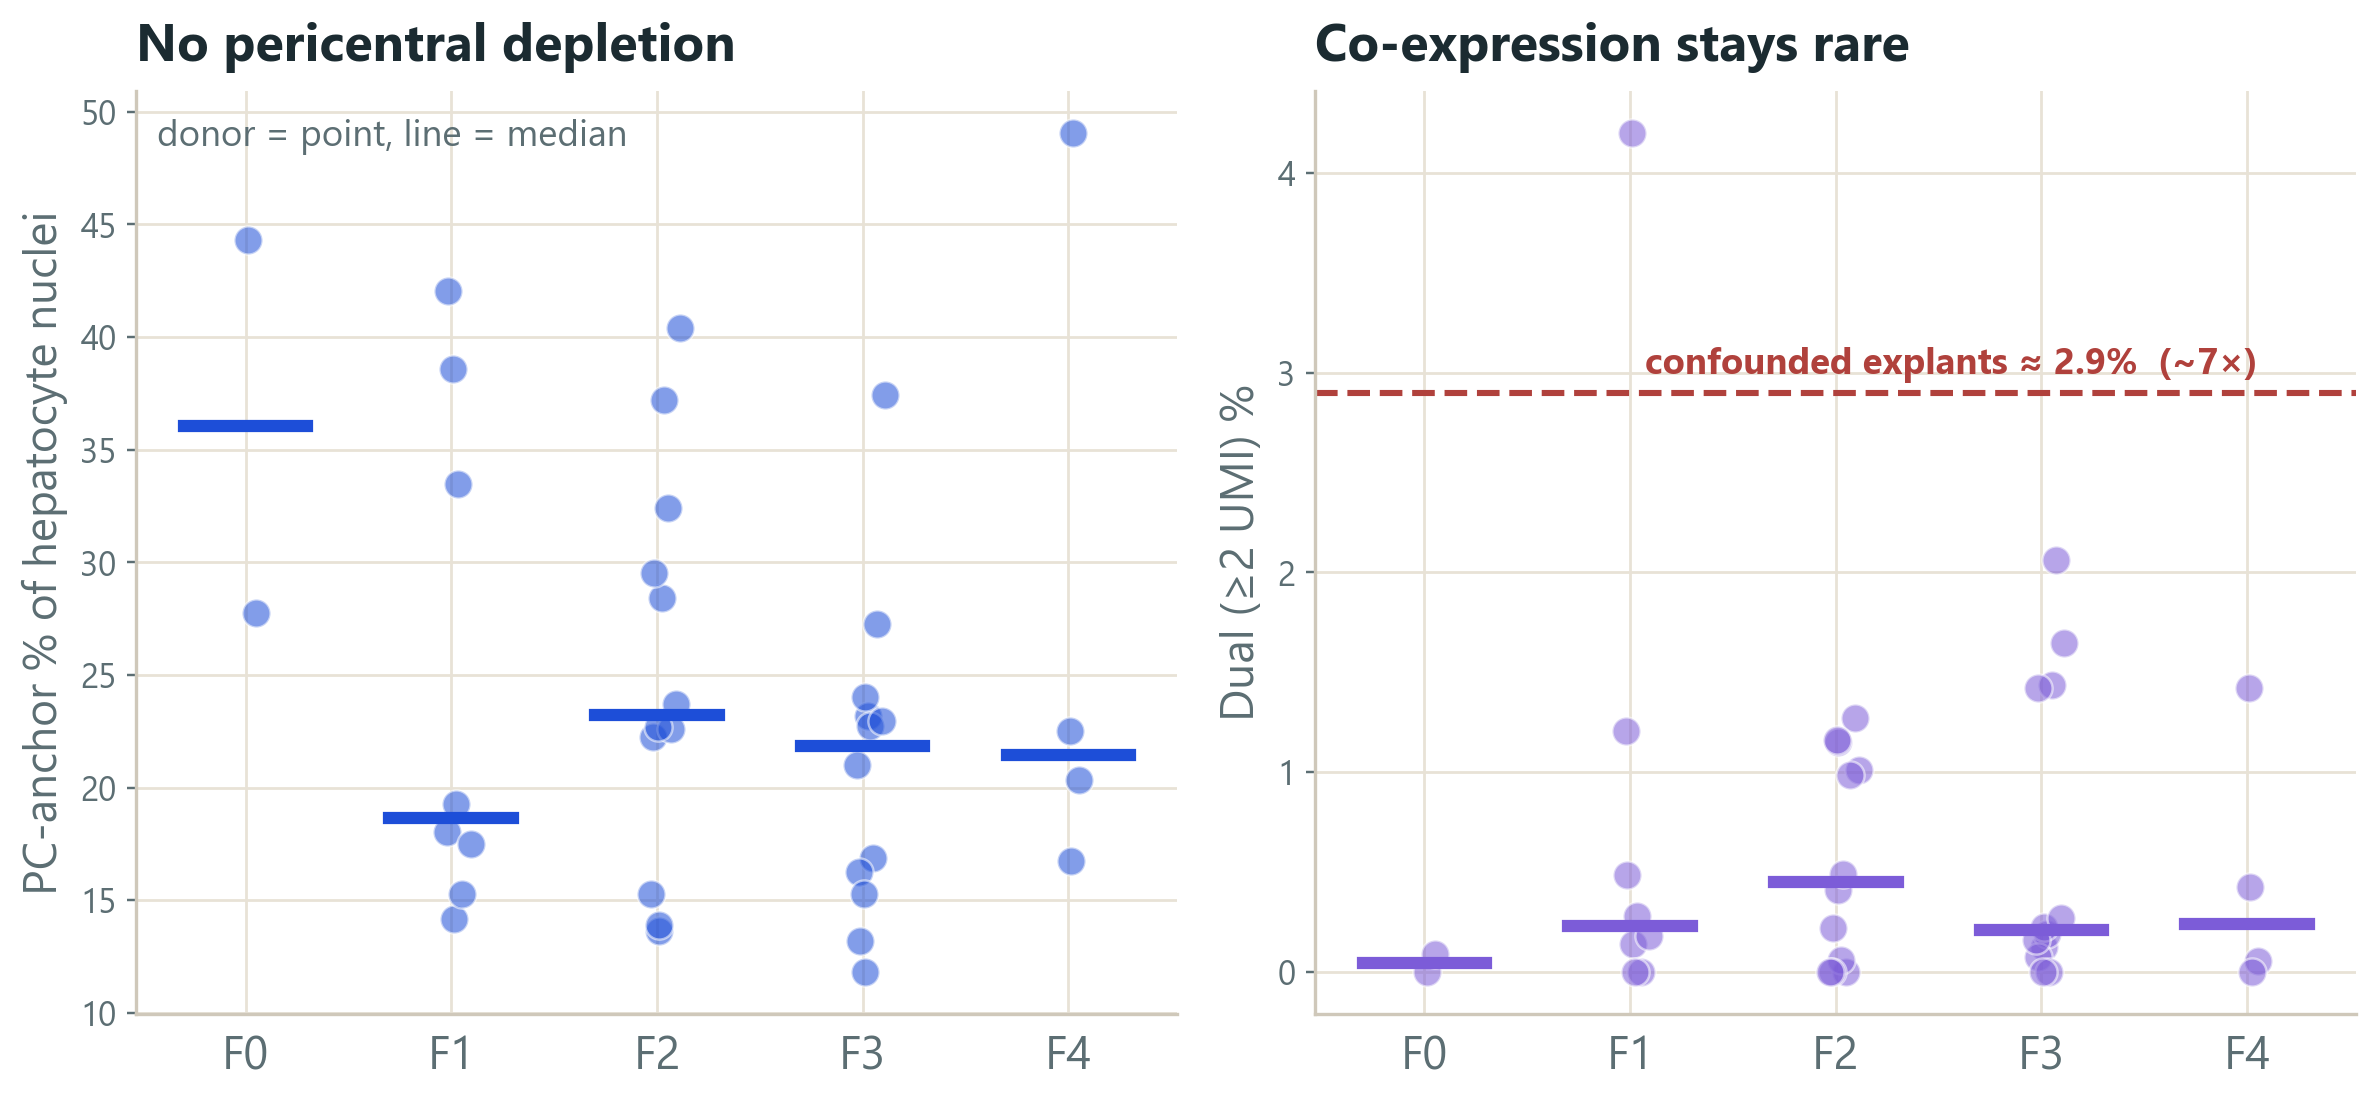
\includegraphics[width=0.8\linewidth]{fig_result2}
\caption{Pericentral-anchor fraction across fibrosis (flat) and the dual co-expression fraction collapsing to $\sim$0 at the $\ge 2$-UMI cut. (See also \texttt{fig\_anchor2x2.png}.)}
\label{fig:result2}
\end{figure}

\subsection{R3 --- Robustness and an honest bound}
The result is stable across the sensitivity grid (depth budgets 1{,}000/1{,}500/3{,}000; GLUL-only/CYP3A4-only/both; Monte-Carlo SD on donor medians 0.006--0.010). An affirmative equivalence test (TOST, 90\% CI, donor-level anchor fractions) puts the F4-vs-F1 PC-anchor change at \textbf{+0.024 (90\% CI $-0.147$ to $+0.194$)}. So we \textbf{exclude a large shift on the order of 20 percentage points} (the well-powered F1$\to$F3 interior tightens to $\sim\pm0.12$); we do \textbf{not} exclude a subtle drift of $\le 10$ points (donor SD is large at F4 n=4). Large re-zonation is ruled out; subtle drift is not.

\begin{figure}[h]
\centering
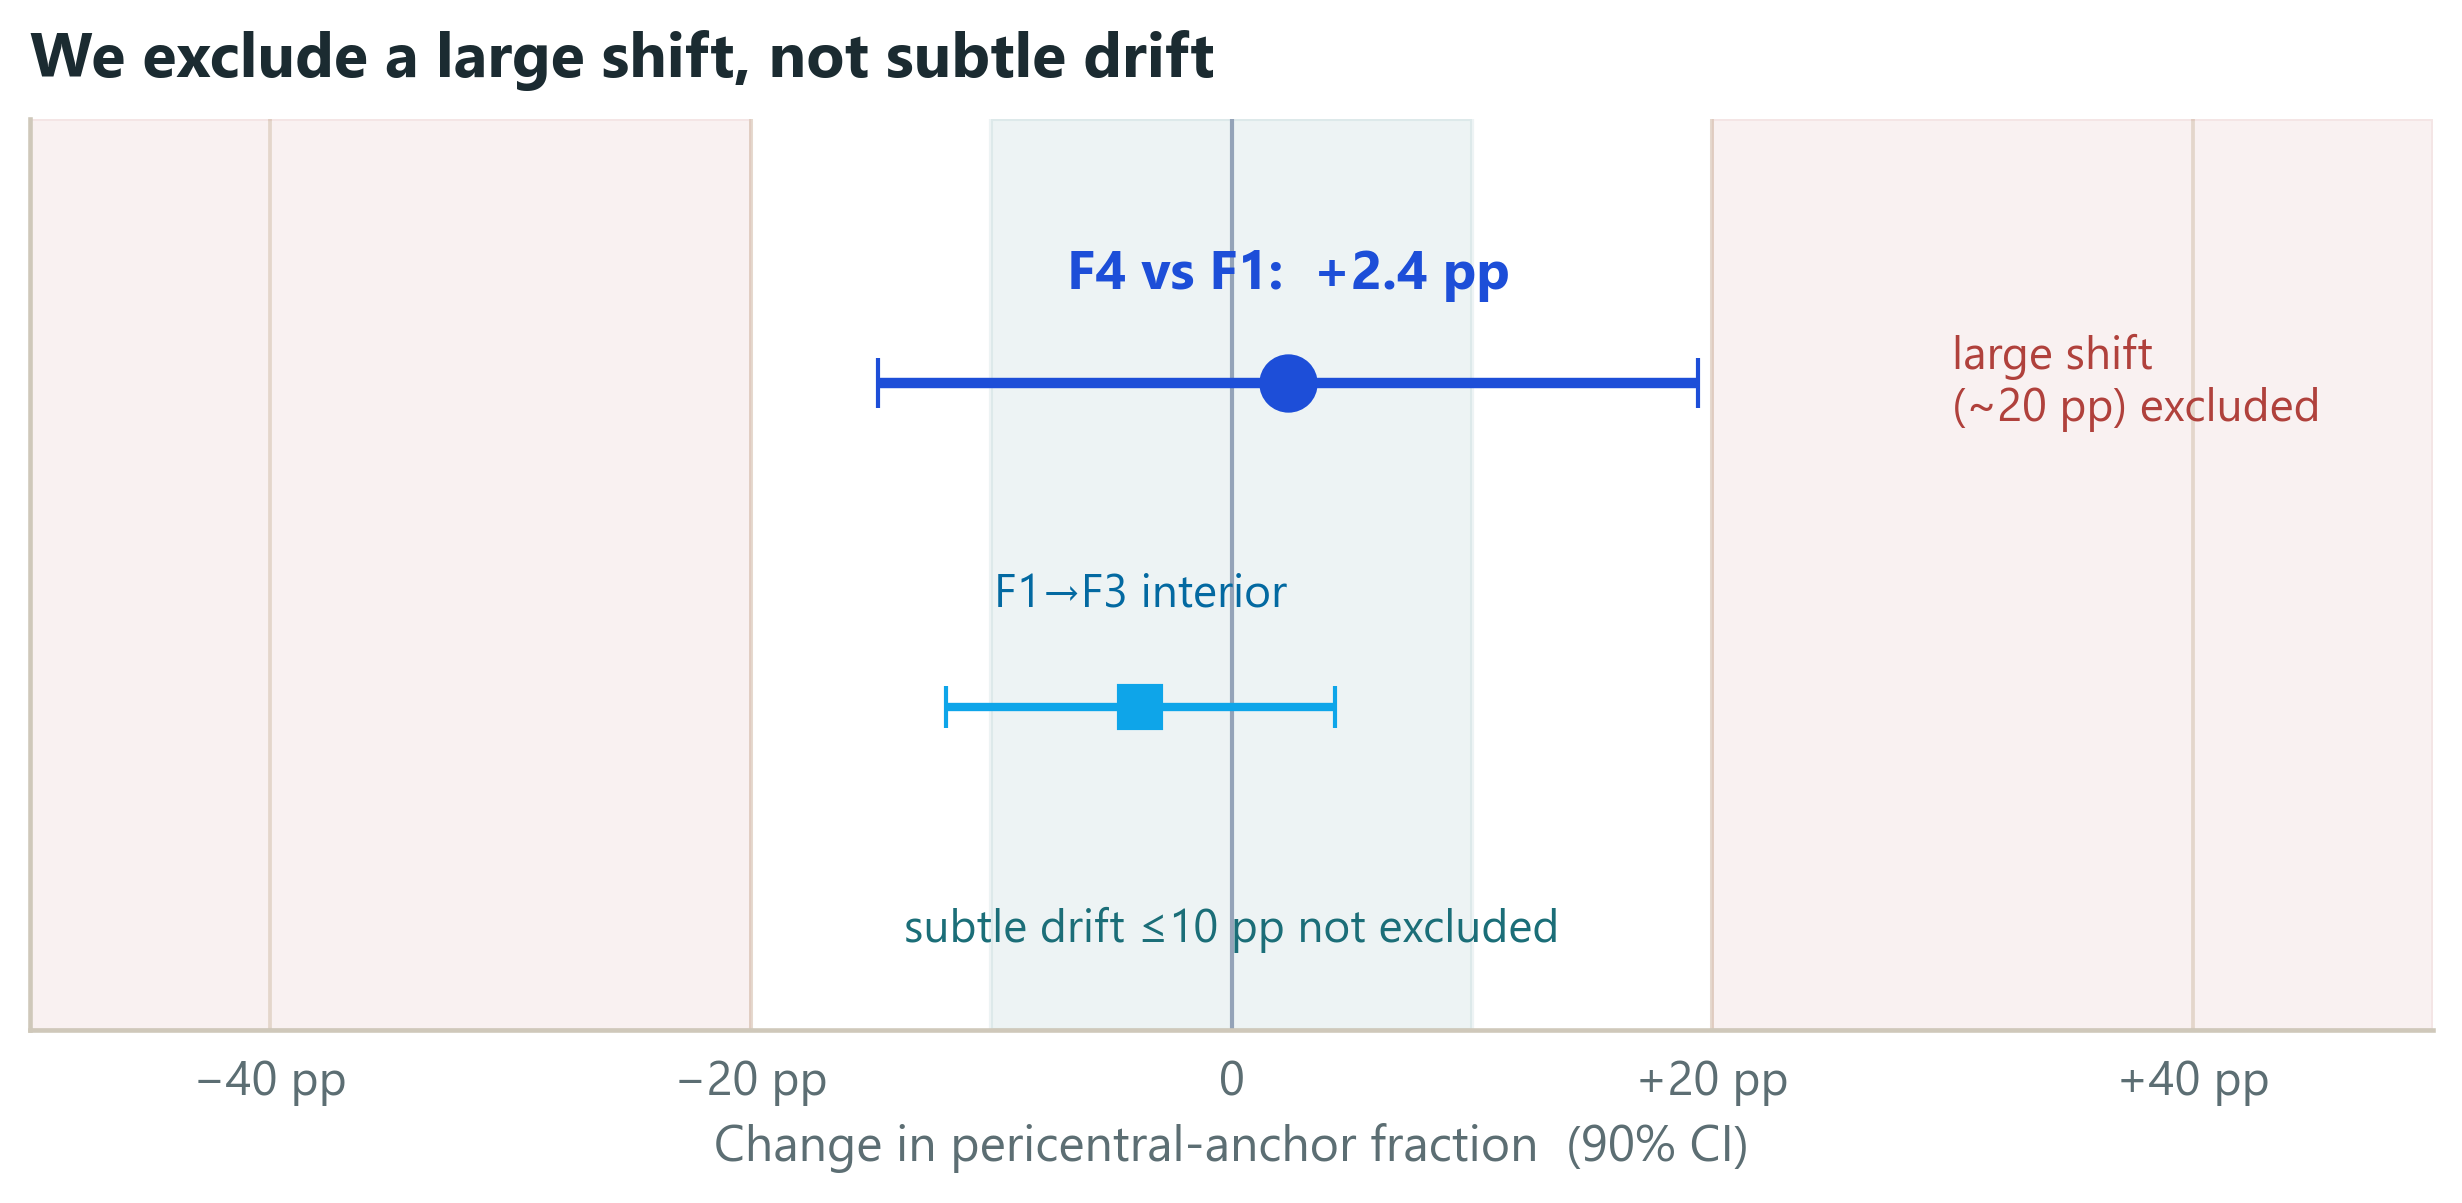
\includegraphics[width=0.8\linewidth]{fig_tost}
\caption{Equivalence bound on the F4-vs-F1 pericentral-anchor change: a large shift is excluded, a subtle one is not.}
\label{fig:tost}
\end{figure}

\subsection{R4 --- The only DGE signal is a biliary burden, likely compositional}
Genome-wide, of $\sim$21{,}000 genes only \textbf{64} reach FDR $< 0.05$ at F4-vs-F1, and they are a biliary/ductular set --- \emph{EPCAM, GRHL2, SPINT2, SOX4, SOX9, B3GNT3} --- plus \emph{CXCL10}. Zonation genes are flat at the expression level (\textbf{GLUL FDR 0.80 --- not significant}; all detox genes FDR $> 0.79$), an independent count-based check agreeing with the anchor classification. So the discovery scan finds \textbf{a biliary-marker burden inside hepatocyte-labeled pseudobulk, not zonation loss.}

Source attribution (a side lead): the headline genes are 5--78$\times$ more abundant in cholangiocytes than hepatocytes; the cholangiocyte fraction rises to $\sim$8\% at F4 (the ductular reaction); only $\sim$0.4\% of hepatocyte nuclei robustly co-express $\ge 2$ biliary markers; ambient correction (decontX) cuts hits 64$\to$34 and drops \emph{SOX4/SOX9} below significance. But \emph{EPCAM/B3GNT3/SPINT2} survive (decontX is a consistency check, not a verdict), and \emph{CXCL10} is separate --- its hepatocyte expression does not track the cholangiocyte fraction (corr $-0.09$), so it is a candidate real inflammatory signal, not ambient. Careful conclusion: the burden is \textbf{real as a signal in hepatocyte-labeled pseudobulk, source not resolved}, and the weight of evidence favors \textbf{ambient RNA + rare mixed/doublet nuclei} over broad transdifferentiation.

\begin{figure}[h]
\centering
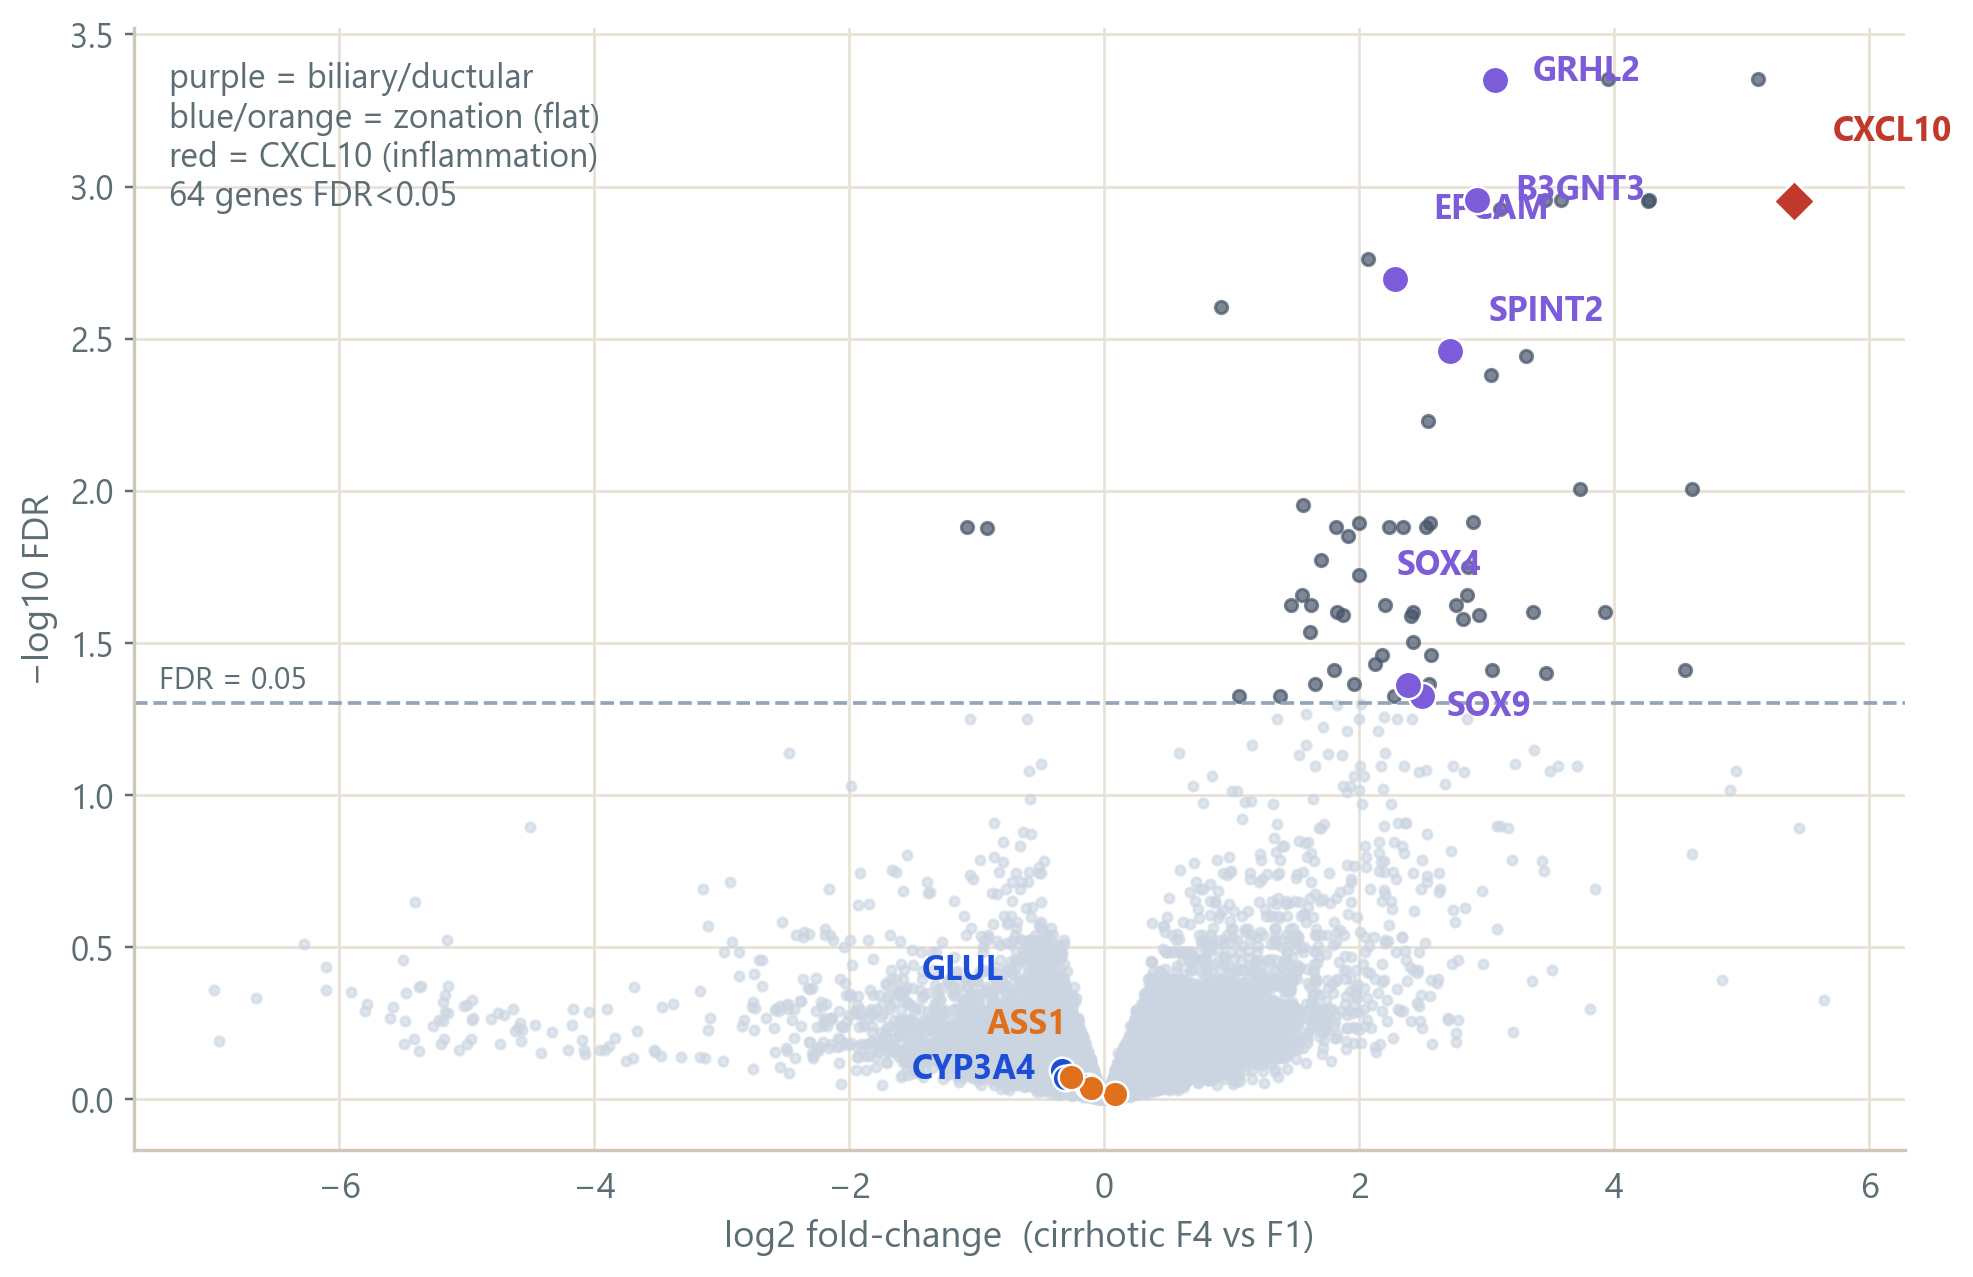
\includegraphics[width=0.8\linewidth]{fig_volcano}
\caption{Volcano (F4-vs-F1): zonation genes flat; the highlighted hits are biliary/ductular markers. Compositional audit places these genes as cholangiocyte-dominant. (\texttt{fig\_volcano.png} + \texttt{fig\_compositional.png}.)}
\label{fig:volcano}
\end{figure}

\FloatBarrier

\section{Interpretation}

\begin{enumerate}[noitemsep]
\item \textbf{The full trajectory is source-confounded} --- do not read healthy $\to$ end-stage as a clean continuation of the disease axis. The endpoints are organ tissue carrying organ-wide procurement stress.
\item \textbf{In matched biopsies, transcriptional zonation is preserved} --- every failure mode (depletion, co-expression, turn-off, composition shift) is flat across F1$\to$cirrhotic F4, and a large coordinated shift is affirmatively excluded.
\item \textbf{The remaining F4 signal is biliary/ductular but source-uncertain} --- most consistent with cholangiocyte ambient RNA plus rare mixed/doublet nuclei, with \emph{CXCL10} a possible real hepatocyte inflammatory exception. This source-attribution leg is a promising lead, not a closed finding.
\end{enumerate}

\section{Limitations and next steps}

Stated plainly, not apologetically. This is a hackathon-scale re-analysis: no wet-lab, no imaging or spatial re-analysis, single cohort. The F4 biopsy stratum is thin (n=4), so subtle effects there are underpowered. Gene-level DGE can miss a \emph{weak coordinated} program in which many genes each shift modestly without any one crossing FDR --- so ``nothing else moves'' carries a gene-level-only caveat. decontX is a sensitivity check using the paper's own labels (mild circularity), not proof of ambient origin. And anchor markers simplify what is really a continuous gradient; snRNA measures per-cell transcriptional balance, not lobule geometry --- we do not claim spatial/architectural preservation.

Next steps: gene-set/pathway tests (CAMERA + ROAST over standard hepatocyte programs) to close the weak-coordinated-program gap; leave-one-F4-donor-out DGE on the biliary hits; a quantitative contamination model asking whether the ambient/doublet burden numerically explains the counts; spatial validation; and an independent MASLD biopsy cohort.

\section*{Appendix / backup}
\addcontentsline{toc}{section}{Appendix / backup}

\begin{sloppypar}
\begin{itemize}
\item \textbf{Why we abandoned the relative ruler.} An early z-scored ``zonation coordinate'' produced an apparent collapse. It was abandoned for two reasons: (a) it pools across the source confound, so a between-group acquisition discontinuity reads as within-group de-zonation (a Simpson's-paradox reversal --- each healthy donor is individually zonated, anti-corr $\approx -0.21$, yet pooling flips the sign to $\approx +0.01$); and (b) it is intrinsically depth-sensitive and mechanism-blind --- turn-off, co-expression, and noise all shrink its spread alike. The count anchor classification separates the mechanisms; the ruler cannot. (\texttt{findings/relative\_ruler\_postmortem/}.)
\item \textbf{End-stage is not one program.} Across the five explants the PC-anchor fraction ranges 3\%$\to$50\% and PP:PC 0.13$\to$20 (CL104 retains pericentral; CL16 collapses to periportal; CL18 floods into co-expression). Pooling five discordant, separately-procured organs into one correlation manufactures a uniform ``collapse.'' (\texttt{reports/SYNTHESIS.md} \S1f.)
\item \textbf{Provenance.} Stress and per-donor maps: \texttt{load\_bearing.py}; cross-lineage stress: \texttt{supplementary\_checks.py}; marker-set invariance: \texttt{all\_sets\_census.py}; genome-wide DGE: \texttt{dge\_genomewide.py} / Plan A \texttt{findings/dge\_plan\_a/}; equivalence bound: \texttt{findings/equivalence\_bound/}. Full numeric record: \texttt{FINDINGS.md} and \texttt{CLAIMS\_LEDGER.md}.
\end{itemize}
\end{sloppypar}

\end{document}
